\chapter{Conclusion Générale et Perspectives d'Évolution}
\label{chap:conclusion}

\section{Bilan des Réalisations Techniques et Scientifiques}

Ce projet de fin d'études a permis de concevoir, développer et valider expérimentalement la plateforme \textbf{Perceptra}, un système complet de recherche d'images par le contenu visuel (CBIR) intégrant un mécanisme d'apprentissage interactif par retour de pertinence (\textit{Relevance Feedback}).

Conformément au cahier des charges académique assigné au \textbf{Groupe 13} par la Faculté des Sciences et Techniques de Tanger, l'intégralité des objectifs a été rigoureusement remplie~:
\begin{enumerate}
    \item \textbf{Gestion Intégrale de Collections Iconographiques~:} Espace applicatif sécurisé autorisant le téléversement individuel et par lots, la détection des doublons par empreinte SHA-256, l'organisation hiérarchique en catégories arborescentes et le filtrage par favoris.
    \item \textbf{Studio de Retouche Géométrique Non Destructif~:} Moteur de transformation (recadrage, rééchantillonnage, rotations orthogonales et continues, matrices affines) préservant l'intégrité de la source originale.
    \item \textbf{Extraction Multi-Facettes Déterministe~:} Famille complète de descripteurs visuels de couleur (histogramme HSV 768-D normalisé L1, moments de couleur 9-D de Stricker \& Orengo, palettes dominantes $K$-Means) et de texture (matrices GLCM de Haralick et motifs LBP 256-D), calculés en moins de 20 millisecondes par image.
    \item \textbf{Contribution Spécifique FRE (Groupe 13)~:} Algorithme d'estimation de pertinence des descripteurs (\textit{Feature Relevance Estimation}) basé sur l'analyse de dispersion intra-classe, le rapport de séparabilité de Fisher, un lissage bayésien avec mémoire d'inertie et la translation adaptative du centroïde de la requête.
    \item \textbf{Architecture Logicielle Moderne et Découplée~:} Backend Flask 3 sous le patron \textit{Service Layer} propulsé par \texttt{uv}, et interface web réactive bâtie sur SvelteKit 3 / Svelte 5 Runes, Shadcn-Svelte, Tailwind CSS 4 et Paraglide-JS.
    \item \textbf{Validation Quantitative Probante~:} Évaluation méthodique sur le jeu \textbf{GHIM-10K} (10\,000 images), démontrant une progression de la précision moyenne $P@10$ de \textbf{58,2\,\%} à \textbf{85,1\,\%} après deux itérations de feedback FRE, soit un gain supérieur à \textbf{26 points de pourcentage}.
\end{enumerate}

\begin{figure}[H]
\centering
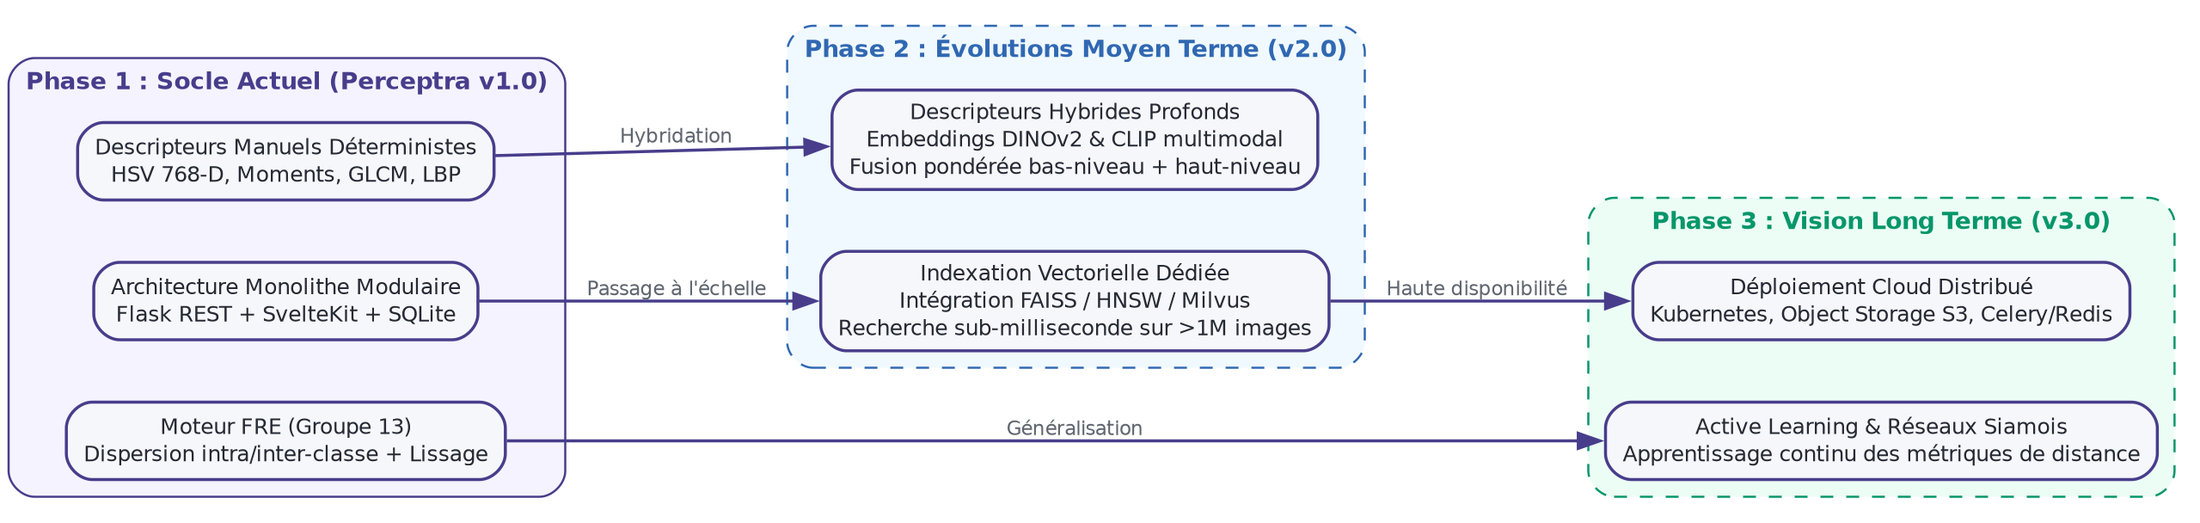
\includegraphics[width=0.78\textwidth]{images/12-cycle-de-vie-et-perspectives.png}
\caption{Feuille de route et perspectives d'évolution architecturale et algorithmique}
\label{fig:perspectives}
\end{figure}

\section{Limites Identifiées et Perspectives d'Avenir}

En dépit de son efficacité démontrée, le système présente un certain nombre de contraintes inhérentes à ses choix fondamentaux de conception~:
\begin{itemize}
    \item \textbf{Scalabilité CPU au-delà du Million d'Images~:} Le moteur actuel opère par balayage vectoriel direct en $\mathcal{O}(N \cdot D)$. Si cette approche est ultra-rapide sur 10\,000 images (38 ms), elle nécessitera une indexation spatiale approximative sur de très grands corpus.
    \item \textbf{Objets Multiples et Échelles Complexes~:} Les descripteurs globaux résumant l'intégralité du champ visuel, un objet d'intérêt occupant une fraction marginale de la scène voit son information diluée dans le fond.
\end{itemize}

Pour dépasser ces frontières et porter Perceptra à l'échelle industrielle, trois perspectives majeures sont engagées~:
\begin{enumerate}
    \item \textbf{Indexation Vectorielle Approchée (ANN) avec FAISS~:} Remplacement du balayage linéaire par des graphes de type \textit{HNSW} pour exécuter des recherches en moins de 5 millisecondes sur plus de 10 millions d'images.
    \item \textbf{Hybridation avec des Représentations Profondes (CLIP \& DINOv2)~:} Fusion pondérée des caractéristiques explicites (GLCM, LBP) avec des embeddings sémantiques profonds issus de transformateurs visuels auto-supervisés.
    \item \textbf{Déploiement Élastique Cloud et Microservices~:} Décomposition en microservices asynchrones sous Kubernetes avec passage d'ordres par files d'attente Redis/Celery.
\end{enumerate}
